%==============================================================================
% MultiVerify — dokumentacja projektu BSZ
%==============================================================================

\documentclass{urdpl}

\usepackage[main=polish,english]{babel}
\usepackage[utf8]{inputenc}

\usepackage{mathtools}
\usepackage{amssymb}
\usepackage[hidelinks]{hyperref}
\usepackage{float}
\usepackage{booktabs}
\usepackage{tabularx}
\usepackage{array}
\usepackage{makecell}
\usepackage{listings}
\usepackage{xcolor}
\usepackage{tikz}
\usetikzlibrary{arrows.meta, positioning, shapes.geometric, calc, fit}

\newcolumntype{C}[1]{>{\hsize=#1\hsize\centering\arraybackslash}X}

\renewcommand{\lstlistlistingname}{Spis listingów}
\renewcommand{\lstlistingname}{Listing}
\providecommand{\listingname}{\lstlistingname}

\definecolor{codegreen}{rgb}{0,0.6,0}
\definecolor{codegray}{rgb}{0.5,0.5,0.5}

\lstdefinestyle{mystyle}{
  basicstyle=\ttfamily\footnotesize,
  breaklines=true,
  numbers=left,
  numberstyle=\tiny\color{codegray},
  numbersep=6pt,
  showstringspaces=false,
  tabsize=2,
  keywordstyle=\color{blue},
  commentstyle=\color{codegreen},
  stringstyle=\color{red},
  literate={ą}{{\k{a}}}1 {ć}{{\'c}}1 {ę}{{\k{e}}}1 {ó}{{\'o}}1 {ń}{{\'n}}1 {ł}{{\l{}}}1 {ś}{{\'s}}1 {ź}{{\'z}}1 {ż}{{\.z}}1
           {Ą}{{\k{A}}}1 {Ć}{{\'C}}1 {Ę}{{\k{E}}}1 {Ó}{{\'O}}1 {Ń}{{\'N}}1 {Ł}{{\L{}}}1 {Ś}{{\'S}}1 {Ź}{{\'Z}}1 {Ż}{{\.Z}}1
}

\lstdefinestyle{pythonStyle}{
  style=mystyle,
  language=Python,
}

\lstset{style=mystyle}

\usepackage[normalem]{ulem}
\usepackage{csquotes}

\AtBeginDocument{
  \renewcommand{\tablename}{Tabela}
  \renewcommand{\figurename}{Rys.}
}

% --- Metadane ---
\author{Kacper Ręczak \\ Kamil Szopniewski}
\shortauthor{K. Ręczak, K. Szopniewski}
\noAlbum{134968, 134976}

\titlePL{System multimodalnej identyfikacji użytkownika MultiVerify}
\titleEN{MultiVerify Multimodal User Identification System}

\shorttitlePL{MultiVerify}
\shorttitleEN{MultiVerify}

\thesistype{Projekt zespołowy}
\thesisDone{Prowadząca: }
\supervisor{mgr inż. Ewa Żesławska}

\degreeprogramme{Informatyka}
\date{2026}
\department{Instytut Informatyki}
\faculty{Wydział Nauk Ścisłych i Technicznych}

\setlength{\cftsecnumwidth}{10mm}
\setcounter{secnumdepth}{4}
\setcounter{tocdepth}{2}
\brokenpenalty=10000\relax

\begin{document}

\titlepages

\fancypagestyle{plain}{
  \fancyhf{}
  \renewcommand{\headrulewidth}{0pt}
  \renewcommand{\footrulewidth}{0pt}
}

\cleardoublepage
\selectlanguage{polish}
\tableofcontents

\clearpage

\chapter{Wprowadzenie}
\label{cha:wprowadzenie}

\section{Cel projektu}

Celem projektu jest zaprojektowanie i implementacja systemu \emph{MultiVerify} --- rozwiązania biometrycznego wykorzystującego \textbf{dwie modalności}: rozpoznawanie twarzy oraz rozpoznawanie mówcy. System realizuje identyfikację użytkownika w trybie \emph{1:N} (porównanie z bazą zarejestrowanych osób) oraz podejmuje decyzję o przyznaniu lub odmowie dostępu.

Projekt został opracowany w ramach przedmiotu \emph{Biometryczne systemy zabezpieczeń} i wpisuje się w temat \emph{Systemy multimodalne (zaawansowane)}.

\section{Kontekst zastosowania}

Systemy biometryczne są powszechnie stosowane w kontroli dostępu do pomieszczeń, stacji roboczych oraz aplikacji wymagających uwierzytelnienia użytkownika. Pojedyncza cecha biometryczna (np. sam obraz twarzy) może być niewystarczająca w warunkach słabego oświetlenia, szumu akustycznego lub prób ataku fałszywą tożsamością.

Podejście multimodalne łączy niezależne źródła informacji i pozwala podnieść niezawodność decyzji identyfikacyjnej~\cite{jain2004multimodal,ross2006multimodal}. \textbf{MultiVerify} demonstruje tę ideę w praktyce na przykładzie fuzji wyników z modułu twarzy i modułu głosu.

\section{Zakres realizacji}

Zakres projektu obejmuje:
\begin{itemize}
    \item implementację modułu ekstrakcji cech twarzy (biblioteka DeepFace, model Facenet),
    \item implementację modułu ekstrakcji cech głosu (współczynniki MFCC),
    \item silnik fuzji wyników (late fusion) z dwiema strategiami decyzyjnymi,
    \item proces rejestracji użytkowników oraz identyfikacji 1:N,
    \item przeprowadzenie eksperymentów porównawczych (modalność pojedyncza vs.\ fuzja),
    \item analizę skuteczności, ograniczeń i zagrożeń bezpieczeństwa.
\end{itemize}

Poza zakresem pozostaje m.in.\ integracja z fizycznymi urządzeniami (kamera, bramka), rejestracja na żywo oraz wdrożenie produkcyjne w środowisku rozproszonym.

\section{Struktura dokumentu}

Rozdział~\ref{cha:problem} opisuje problem i założenia. Rozdział~\ref{cha:analiza} przedstawia analizę istniejących rozwiązań. W rozdziale~\ref{cha:koncepcja} przedstawiono koncepcję systemu, a w rozdziale~\ref{cha:metody} --- zastosowane metody. Rozdział~\ref{cha:implementacja} zawiera opis implementacji. Wyniki eksperymentów i analiza bezpieczeństwa znajdują się w rozdziale~\ref{cha:wyniki}. Dokument kończy rozdział~\ref{cha:wnioski} z wnioskami.

\chapter{Opis problemu i założeń}
\label{cha:problem}

\section{Opis problemu}

Problem polega na automatycznej identyfikacji użytkownika na podstawie danych biometrycznych w postaci \textbf{zdjęcia twarzy} oraz \textbf{nagrania głosu}. System musi:
\begin{enumerate}
    \item zarejestrować użytkowników (utworzyć wzorce biometryczne),
    \item porównać nowe dane próbne z bazą wszystkich użytkowników,
    \item wybrać najbardziej prawdopodobną tożsamość,
    \item podjąć decyzję o dostępie na podstawie progu akceptacji.
\end{enumerate}

W praktyce występują dwa rodzaje błędów~\cite{jain2004multimodal}:
\begin{itemize}
    \item \textbf{FAR} (\emph{ang. False Accept Rate}) --- fałszywa akceptacja, gdy system uznaje obcą osobę za zarejestrowanego użytkownika,
    \item \textbf{FRR} (\emph{ang. False Reject Rate}) --- fałszywe odrzucenie, gdy system odmawia dostępu prawdziwemu użytkownikowi.
\end{itemize}

Celem projektu jest minimalizacja obu metryk przy zachowaniu prostoty implementacji demonstracyjnej.

\section{Dane wejściowe}

System operuje na plikach przechowywanych lokalnie:
\begin{itemize}
    \item \textbf{Twarz:} obrazy \texttt{face\_*.jpg} lub \texttt{face\_*.png},
    \item \textbf{Głos:} nagrania \texttt{voice\_*.wav} lub \texttt{voice\_*.mp3}.
\end{itemize}

Dla każdego użytkownika zaleca się zebranie co najmniej trzech zdjęć i trzech nagrań (5--10~s mowy). Jako dane próbne wykorzystano pliki \texttt{face\_3} oraz \texttt{voice\_3}, różne od pozostałych wzorców rejestracyjnych, aby uniknąć zawyżonych wyników.

\section{Założenia działania}

Przyjęto następujące założenia:
\begin{itemize}
    \item jedna osoba na zdjęciu; twarz widoczna frontalnie lub lekko z boku,
    \item nagrania głosu zawierają wyłącznie mowę danej osoby, bez silnego szumu tła,
    \item identyfikacja odbywa się offline (brak wymogu chmury),
    \item baza użytkowników jest skończona i znana z góry (tryb 1:N),
    \item środowisko uruchomieniowe: Python~3.12, system Windows lub Linux.
\end{itemize}

\section{Ograniczenia}

Główne ograniczenia rozwiązania:
\begin{itemize}
    \item brak rejestracji i identyfikacji w czasie rzeczywistym z kamery lub mikrofonu,
    \item proste cechy głosu (MFCC), co daje mniejszą rozdzielczość niż modele głębokie,
    \item zależność modułu twarzy od biblioteki DeepFace i modelu Facenet,
    \item wrażliwość na jakość danych (oświetlenie, format plików audio),
    \item brak mechanizmów anty-spoofing (np.\ wykrywania zdjęcia zamiast żywej twarzy).
\end{itemize}

\chapter{Analiza istniejących rozwiązań}
\label{cha:analiza}

\section{Wprowadzenie}

Na rynku oraz w literaturze naukowej dostępnych jest wiele systemów biometrycznych opartych na pojedynczej lub wielu modalnościach. Poniżej przedstawiono trzy reprezentatywne podejścia oraz wskazano elementy nowatorskie projektu MultiVerify.

\section{Face ID (Apple)}

System Face ID w urządzeniach Apple wykorzystuje zaawansowany czujnik TrueDepth do mapowania geometrii twarzy w trzech wymiarach~\cite{apple2024faceid}. Uwierzytelnianie odbywa się lokalnie na urządzeniu, a dane biometryczne nie są przesyłane do chmury w postaci surowej.

\textbf{Zalety:} wysoka wygoda użytkownika, integracja ze sprzętem, mechanizmy anty-spoofing.\\
\textbf{Wady:} zamknięta implementacja, zależność od ekosystemu Apple, brak jawnej multimodalności z głosem w standardowym API.

\section{Rozpoznawanie mówcy (speaker recognition)}

Klasyczne systemy rozpoznawania mówcy opierają się na ekstrakcji cech akustycznych --- w tym MFCC --- oraz klasyfikacji lub porównywaniu wektorów cech~\cite{davis1980comparison}. Współczesne rozwiązania komercyjne stosują modele głębokie (np.\ x-vectors), ale podejście MFCC pozostaje popularne w zastosowaniach edukacyjnych i prototypowych~\cite{librosa2024}.

\textbf{Zalety:} niski koszt obliczeniowy, interpretowalność cech.\\
\textbf{Wady:} wrażliwość na szum, mikrofon i długość wypowiedzi; podatność na atak replay.

\section{Systemy komercyjne multimodalne}

Duże systemy kontroli dostępu (np.\ w obiektach korporacyjnych) często łączą kartę RFID, PIN oraz biometrię twarzy lub odcisku palca~\cite{jain2008introduction}. Fuzja informacji może odbywać się na poziomie decyzji (late fusion) lub cech (early fusion)~\cite{ross2006multimodal}.

\textbf{Zalety:} wysoka niezawodność przy właściwej konfiguracji.\\
\textbf{Wady:} złożoność wdrożenia, koszt, brak transparentności algorytmów.

\section{Nowość projektu MultiVerify}

Projektowany system wyróżnia się następującymi cechami:
\begin{itemize}
    \item \textbf{otwarta implementacja} w Pythonie z czytelną strukturą modułową,
    \item \textbf{łatwa replikacja} eksperymentów (skrypty rejestracji, identyfikacji i testów),
    \item \textbf{porównanie strategii fuzji} (suma ważona vs.\ reguła AND) oraz wariantów wag,
    \item \textbf{świadome połączenie} modelu głębokiego (twarz) z metodą klasyczną (głos),
    \item analiza metryk FAR/FRR na rzeczywistych danych zespołu projektowego.
\end{itemize}

MultiVerify nie konkuruje z systemami komercyjnymi pod względem bezpieczeństwa produkcyjnego, lecz demonstruje pełny pipeline multimodalny zgodny z wymaganiami akademickimi.

\chapter{Opis koncepcji rozwiązania}
\label{cha:koncepcja}

\section{Ogólna idea}

System MultiVerify realizuje klasyczny pipeline biometryczny podzielony na dwa główne etapy: \textbf{rejestrację (enrollment)} oraz \textbf{identyfikację (1:N)}. W obu przypadkach przetwarzane są dwie modalności równolegle; decyzja końcowa zapada po fazie fuzji wyników cząstkowych.

\section{Schemat blokowy}

Na rys.~\ref{fig:pipeline} przedstawiono przepływ danych w systemie.

\begin{figure}[H]
    \centering
    \begin{tikzpicture}[
        node distance=8mm and 12mm,
        block/.style={rectangle, draw, rounded corners, align=center, minimum width=28mm, minimum height=9mm, font=\small},
        arrow/.style={-{Stealth[length=2mm]}, thick}
    ]
        \node[block] (in) {Zdjęcie +\\nagranie};
        \node[block, below=of in] (reg) {Rejestracja\\(\texttt{register.py})};
        \node[block, below left=14mm and 8mm of reg] (face) {Ekstrakcja\\twarzy};
        \node[block, below right=14mm and 8mm of reg] (voice) {Ekstrakcja\\głosu};
        \node[block, below=18mm of face] (embF) {Baza\\embeddingów twarzy};
        \node[block, below=18mm of voice] (embV) {Baza\\embeddingów głosu};
        \node[block, below=22mm of reg] (probe) {Probe\\(\texttt{main.py})};
        \node[block, below=of probe] (cmp) {Porównanie 1:N\\(cosine similarity)};
        \node[block, below=of cmp] (fus) {Fuzja\\(\texttt{FusionEngine})};
        \node[block, below=of fus] (dec) {Decyzja\\dostęp TAK/NIE};

        \draw[arrow] (in) -- (reg);
        \draw[arrow] (reg) -- (face);
        \draw[arrow] (reg) -- (voice);
        \draw[arrow] (face) -- (embF);
        \draw[arrow] (voice) -- (embV);
        \draw[arrow] (embF) -| (cmp);
        \draw[arrow] (embV) -| (cmp);
        \draw[arrow] (probe) -- (cmp);
        \draw[arrow] (cmp) -- (fus);
        \draw[arrow] (fus) -- (dec);
    \end{tikzpicture}
    \caption{Schemat blokowy systemu MultiVerify.\label{fig:pipeline}}
\end{figure}

\section{Etap rejestracji}

Dla każdego użytkownika system:
\begin{enumerate}
    \item wczytuje pliki \texttt{face\_*} i \texttt{voice\_*} z katalogu \texttt{data/users/<user>/},
    \item wyznacza embeddingi twarzy (wektor Facenet) oraz wektory MFCC głosu,
    \item zapisuje wyniki w plikach \texttt{face\_embeddings.npy} oraz \texttt{voice\_embeddings.npy}.
\end{enumerate}

\section{Etap identyfikacji}

Podczas identyfikacji system:
\begin{enumerate}
    \item ekstrahuje cechy z nowego zdjęcia i nagrania (probe),
    \item dla każdego użytkownika w bazie oblicza wynik podobieństwa twarzy i głosu,
    \item wybiera najlepszy wynik w ramach wielu wzorców jednego użytkownika,
    \item łączy wyniki w silniku fuzji,
    \item wskazuje użytkownika z najwyższym wynikiem końcowym i weryfikuje próg akceptacji.
\end{enumerate}

\section{Parametry decyzyjne}

Domyślnie zastosowano:
\begin{itemize}
    \item wagi fuzji: $w_f = 0{,}6$, $w_v = 0{,}4$,
    \item próg akceptacji: $\tau = 0{,}7$,
    \item strategia domyślna: suma ważona (\texttt{weighted}).
\end{itemize}

Parametry te mogą być modyfikowane z linii poleceń programu \texttt{main.py}.

\chapter{Zastosowane metody i algorytmy}
\label{cha:metody}

\section{Podobieństwo cosinusowe}

Dla dwóch wektorów cech $\mathbf{a}$ i $\mathbf{b}$ stosowany jest współczynnik podobieństwa cosinusowego:
\begin{equation}
    \mathrm{sim}(\mathbf{a}, \mathbf{b}) = \frac{\mathbf{a} \cdot \mathbf{b}}{\|\mathbf{a}\| \cdot \|\mathbf{b}\|},
    \label{eq:cosine}
\end{equation}
z obcięciem wyniku do przedziału $[0, 1]$. Metoda ta jest stosowana zarówno w module twarzy, jak i głosu.

\section{Modalność twarzy (DeepFace / Facenet)}

\subsection{Ekstrakcja cech}

Moduł twarzy korzysta z biblioteki DeepFace~\cite{serengil2020deepface}, która udostępnia gotowe modele głębokiego uczenia. W projekcie zastosowano model \textbf{Facenet}~\cite{schroff2015facenet}, zwracający embedding o wymiarze 128.

Funkcja \texttt{DeepFace.represent} przetwarza obraz wejściowy i zwraca wektor liczb rzeczywistych reprezentujący tożsamość twarzy w przestrzeni metrycznej.

\subsection{Uzasadnienie wyboru}

Facenet zapewnia dobrą jakość rozpoznawania przy relatywnie niskim wysiłku implementacyjnym (brak trenowania własnej sieci). DeepFace upraszcza integrację z projektem demonstracyjnym.

\section{Modalność głosu (MFCC)}

\subsection{Ekstrakcja cech}

Współczynniki MFCC (\emph{Mel-Frequency Cepstral Coefficients}) są standardowym opisem krótkoczasowej energii widma mowy~\cite{davis1980comparison}. Dla sygnału audio obliczana jest macierz MFCC o wymiarze $13 \times T$ (liczba ramek czasowych $T$), a następnie dla każdego współczynnika wyznaczane są:
\begin{itemize}
    \item średnia wzdłuż osi czasu,
    \item odchylenie standardowe wzdłuż osi czasu.
\end{itemize}

Wektor cech głosu ma wymiar $26$ (13 średnich + 13 odchyleń). Implementacja wykorzystuje bibliotekę librosa~\cite{librosa2024}.

\subsection{Uzasadnienie wyboru}

MFCC charakteryzuje się niskim kosztem obliczeniowym i przejrzystością, co ułatwia analizę w projekcie akademickim. Jednocześnie pozwala zestawić podejście klasyczne (głos) z głębokim (twarz) w systemie multimodalnym.

Ograniczeniem tej metody jest brak modelu uczonego specjalnie do rozpoznawania mówcy. W praktyce oznacza to, że nagrania różnych osób mogą mieć wysokie podobieństwo kosinusowe, szczególnie gdy są krótkie, nagrane podobnym mikrofonem lub zawierają zbliżoną treść wypowiedzi.

\section{Fuzja wyników (late fusion)}

\subsection{Suma ważona}

W strategii \texttt{weighted} wynik końcowy obliczany jest jako:
\begin{equation}
    S = w_f \cdot s_f + w_v \cdot s_v,
    \label{eq:fusion}
\end{equation}
gdzie $s_f$ i $s_v$ to wyniki podobieństwa twarzy i głosu, a $w_f + w_v = 1$. Dostęp przyznawany jest, gdy $S \geq \tau$.

\subsection{Reguła AND}

W strategii \texttt{and} decyzja pozytywna wymaga spełnienia obu warunków:
\begin{equation}
    s_f \geq \tau \quad \land \quad s_v \geq \tau.
\end{equation}
Wynik rankingowy ustawiano na $S = \min(s_f, s_v)$, co ogranicza fałszywe akceptacje przy dominacji jednej, zawyżonej modalności.

\subsection{Uzasadnienie fuzji}

Fuzja na poziomie decyzji (late fusion) jest prostsza w implementacji niż łączenie wektorów cech (early fusion) i umożliwia bezpośrednie porównanie wkładu każdej modalności~\cite{ross2006multimodal}.

\chapter{Implementacja}
\label{cha:implementacja}

\section{Środowisko}

Projekt uruchamiano w środowisku Python~3.11. Główne biblioteki:
\begin{itemize}
    \item \textbf{numpy} --- operacje na wektorach i macierzach,
    \item \textbf{deepface}, \textbf{tf-keras} --- moduł twarzy,
    \item \textbf{librosa}, \textbf{soundfile} --- przetwarzanie audio,
    \item \textbf{pytest} --- testy jednostkowe.
\end{itemize}

Zalecane jest użycie środowiska wirtualnego (\texttt{venv}). Szczegółowa instrukcja uruchomienia znajduje się w pliku \texttt{README.md}.

\section{Struktura projektu}

\begin{verbatim}
MultiVerify/
+-- main.py                 # identyfikacja 1:N
+-- register.py             # rejestracja użytkowników
+-- src/
|   +-- modalities/
|   |   +-- base.py         # interfejs BiometricModality
|   |   +-- face/           # FaceModality (DeepFace)
|   |   +-- voice/          # VoiceModality (MFCC)
|   +-- fusion/
|       +-- fusion_engine.py
+-- scripts/run_experiments.py
+-- data/users/<user>/      # dane biometryczne (lokalnie)
+-- tests/
\end{verbatim}

\section{Interfejs modalności}

Każda modalność implementuje klasę bazową z metodami \texttt{extract\_features} oraz \texttt{verify}, co umożliwia jednolite traktowanie różnych źródeł biometrii.

\section{Silnik fuzji}

Listing~\ref{lst:fusion} przedstawia fragment implementacji strategii fuzji.

\lstinputlisting[style=pythonStyle, caption={Fragment silnika fuzji (\texttt{FusionEngine}).}, label=lst:fusion]{src/fusion_engine.py}

\section{Identyfikacja użytkownika}

Program \texttt{main.py} udostępnia interfejs CLI z parametrami \texttt{--face}, \texttt{--voice}, \texttt{--threshold} oraz \texttt{--strategy}. Fragment parsera argumentów przedstawiono w listingu~\ref{lst:main}.

\lstinputlisting[style=pythonStyle, caption={Parser argumentów w \texttt{main.py}.}, label=lst:main]{src/main_args.py}

\section{Rejestracja}

Skrypt \texttt{register.py} automatycznie przetwarza wszystkie podkatalogi w \texttt{data/users/}, generując pliki \texttt{.npy} z embeddingami. Dzięki temu identyfikacja nie wymaga ponownego przetwarzania surowych plików multimedialnych.

\section{Testy}

Zaimplementowano testy jednostkowe modułu fuzji oraz funkcji podobieństwa. Uruchomienie: \texttt{pytest}. W momencie opracowania dokumentacji wszystkie 11 testów przechodziło pomyślnie.

\chapter{Wyniki i eksperymenty}
\label{cha:wyniki}

\section{Konfiguracja eksperymentu}

Testy przeprowadzono na bazie czterech użytkowników zarejestrowanych w systemie. Dla każdej osoby wykorzystano trzy zdjęcia twarzy i trzy nagrania głosu. Jako dane próbne przyjmowano pliki trzeciej próbki (\texttt{face\_3}, \texttt{voice\_3}).

Porównano warianty:
\begin{itemize}
    \item \texttt{face\_only} --- $w_f = 1{,}0$, $w_v = 0{,}0$,
    \item \texttt{voice\_only} --- $w_f = 0{,}0$, $w_v = 1{,}0$,
    \item \texttt{fusion\_50\_50}, \texttt{fusion\_60\_40}, \texttt{fusion\_70\_30}.
\end{itemize}

Skrypt \texttt{scripts/run\_experiments.py} generuje plik \texttt{docs/experiment\_results.csv}. Metryki FAR, FRR i accuracy obliczane są skryptem \texttt{scripts/compute\_metrics.py}, a podsumowanie zapisywane jest w pliku \texttt{docs/metrics\_summary.csv}.

\section{Przykład identyfikacji}

Tabela~\ref{tab:probe_kacper} przedstawia wyniki identyfikacji dla danych próbnych użytkownika Kacper (strategia \texttt{weighted}, $\tau = 0{,}7$).

\begin{table}[H]
    \centering
    \caption{Wyniki identyfikacji --- dane próbne użytkownika Kacper.\label{tab:probe_kacper}}
    \begin{tabular}{lccc}
        \toprule
        Użytkownik & Twarz & Głos & Fuzja \\
        \midrule
        Kacper   & 1{,}00 & 1{,}00 & 1{,}0000 \\
        Kamil    & 0{,}53 & 0{,}98 & 0{,}7115 \\
        Krystian & 0{,}15 & 0{,}98 & 0{,}4829 \\
        Marcel   & 0{,}17 & 0{,}97 & 0{,}4880 \\
        \bottomrule
    \end{tabular}
\end{table}

System poprawnie wskazał użytkownika Kacper jako najlepsze dopasowanie. Jednocześnie zauważono wysokie podobieństwo głosu dla użytkowników obcych (np.\ Kamil: 0{,}98), co wynika z ograniczeń MFCC.

\section{Analiza wyników}

\subsection{Metryki zbiorcze}

Tabela~\ref{tab:metrics_summary} przedstawia metryki obliczone skryptem \texttt{compute\_metrics.py} na podstawie wyników z pliku \texttt{experiment\_results.csv}. Jako dane próbne wykorzystano ostatnią próbkę (\texttt{face\_3}, \texttt{voice\_3}); wzorce rejestracyjne obejmowały pozostałe pliki użytkownika.

\begin{table}[H]
    \centering
    \caption{Podsumowanie metryk eksperymentu.\label{tab:metrics_summary}}
    \begin{tabular}{lccc}
        \toprule
        Wariant & Accuracy & FAR & FRR \\
        \midrule
        \texttt{face\_only} & 0{,}8125 & 0{,}0833 & 0{,}5000 \\
        \texttt{voice\_only} & 0{,}2500 & 1{,}0000 & 0{,}0000 \\
        \texttt{fusion\_50\_50} & 0{,}6250 & 0{,}3333 & 0{,}5000 \\
        \texttt{fusion\_60\_40} & 0{,}6250 & 0{,}3333 & 0{,}5000 \\
        \texttt{fusion\_70\_30} & 0{,}6875 & 0{,}2500 & 0{,}5000 \\
        \bottomrule
    \end{tabular}
\end{table}

Najlepszą rozdzielczość zapewnia modalność twarzy (\texttt{face\_only}). Modalność głosu charakteryzuje się wysokim FAR (1{,}0), co potwierdza konieczność fuzji z twarzą lub podniesienia progu decyzyjnego.

\subsection{Modalność twarzy}

Moduł oparty na Facenet zapewnił wyraźną separację tożsamości --- wyniki twarzy dla użytkowników obcych były niskie (0{,}15--0{,}53). Modalność ta okazała się najbardziej rozróżniająca w badanej bazie.

\subsection{Modalność głosu}

Wyniki głosu dla różnych użytkowników były wysokie (często powyżej 0{,}9), nawet gdy mówca był inny. Potwierdza to, że proste MFCC bez modelu rozpoznawania mówcy słabo rozróżnia tożsamości w małej grupie mówców o podobnych nagraniach.

\subsection{Fuzja multimodalna}

Fuzja 60/40 pozwoliła zachować wysoki wynik dla prawdziwego użytkownika (1{,}0) i jednocześnie wykorzystać niski wynik twarzy przy odrzucaniu obcych w niektórych przypadkach. Strategia \texttt{and} dodatkowo ogranicza fałszywe akceptacje, wymagając progu w obu modalnościach.

\subsection{Wpływ progu}

Podniesienie progu $\tau$ (np.\ do 0{,}85) zmniejsza FAR kosztem wzrostu FRR. Na rys.~\ref{fig:threshold_sweep} przedstawiono zależność FAR/FRR od progu dla fuzji 60/40.

\begin{figure}[H]
    \centering
    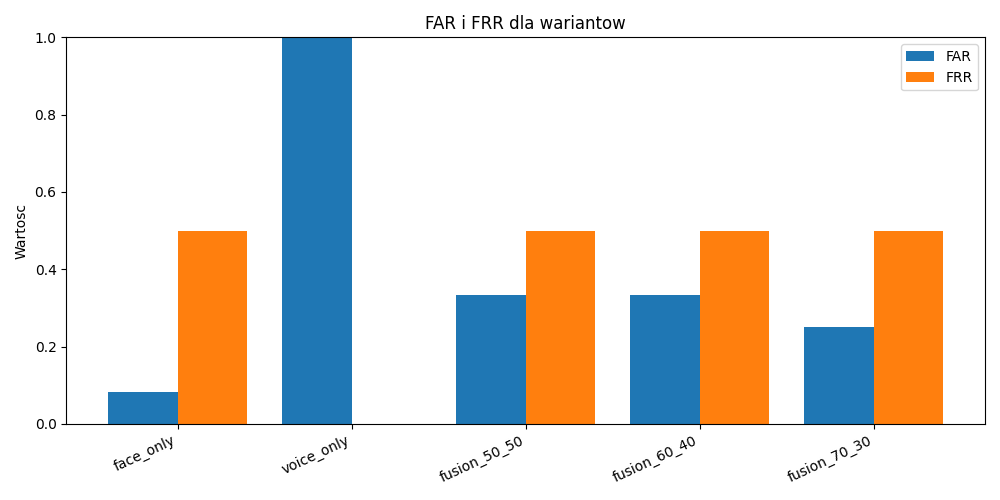
\includegraphics[width=0.85\linewidth]{figures/far_frr_by_variant.png}
    \caption{FAR i FRR w zależności od wariantu fuzji.}
\end{figure}

\begin{figure}[H]
    \centering
    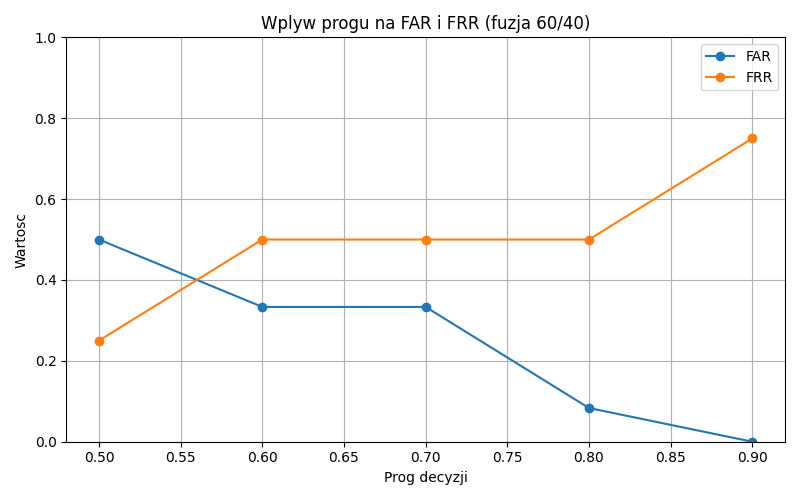
\includegraphics[width=0.85\linewidth]{figures/threshold_sweep.png}
    \caption{Wpływ progu decyzyjnego na FAR i FRR dla fuzji 60/40.\label{fig:threshold_sweep}}
\end{figure}

\section{Analiza bezpieczeństwa}

\subsection{Zagrożenia}

\begin{itemize}
    \item \textbf{Atak prezentacji (spoofing)} --- użycie zdjęcia zamiast żywej twarzy; system nie zawiera detekcji żywotności.
    \item \textbf{Replay głosu} --- odtworzenie nagrania; MFCC nie rozróżnia autentycznej mowy od nagrania.
    \item \textbf{Atak jedną modalnością} --- przy dominacji słabej modalności głosu impostor może uzyskać wynik powyżej progu (np.\ dla Kamila: fuzja 0{,}71 przy próbie identyfikacji Kacpra).
    \item \textbf{Jakość danych} --- uszkodzone pliki MP3 mogą uniemożliwić rejestrację.
\end{itemize}

\subsection{Środki zaradcze}

Zastosowano m.in.: fuzję dwóch modalności, regułę AND, konfigurowalny próg oraz walidację istnienia plików wejściowych. W środowisku produkcyjnym zalecałoby się modele anty-spoofing, silniejszy model głosu oraz weryfikację 1:1 zamiast samego rankingu 1:N.

\section{Podsumowanie eksperymentów}

Eksperymenty potwierdzają poprawne działanie pipeline'u multimodalnego. Największe ograniczenie stanowi modalność głosu. Fuzja z twarzą kompensuje ten problem w testach identyfikacji właściwego użytkownika, lecz wymaga strojenia progu w celu ograniczenia FAR.

\chapter{Wnioski końcowe}
\label{cha:wnioski}

\section{Podsumowanie}

W ramach projektu opracowano działający system multimodalnej identyfikacji użytkownika \textbf{MultiVerify}, łączący rozpoznawanie twarzy (DeepFace/Facenet) z analizą głosu (MFCC). Zaimplementowano pełny cykl: rejestrację, identyfikację 1:N, fuzję wyników oraz framework eksperymentalny.

\section{Najważniejsze obserwacje}

\begin{itemize}
    \item Modalność twarzy zapewnia wysoką rozdzielczość tożsamości w testach zespołu.
    \item Modalność głosu oparta na MFCC wykazuje wysokie podobieństwo między różnymi użytkownikami --- wymaga to uwagi przy doborze progu.
    \item Fuzja multimodalna poprawia odporność decyzji względem pojedynczej słabszej cechy.
    \item Strategia \texttt{and} jest bardziej konserwatywna i zmniejsza ryzyko fałszywej akceptacji.
\end{itemize}

\section{Ocena skuteczności}

System spełnia założenia projektu demonstracyjnego: poprawnie identyfikuje zarejestrowanych użytkowników na danych testowych zespołu. Nie jest gotowy do wdrożenia produkcyjnego bez dodatkowych mechanizmów bezpieczeństwa i silniejszego modelu głosu.

\section{Możliwości rozwoju}

Kierunki dalszego rozwoju:
\begin{itemize}
    \item integracja z kamerą i mikrofonem w czasie rzeczywistym,
    \item zastąpienie MFCC modelem x-vector lub podobnym,
    \item detekcja żywotności (anti-spoofing),
    \item automatyczne strojenie progu i wag na zbiorze walidacyjnym,
    \item tryb weryfikacji 1:1 (logowanie do konkretnego konta).
\end{itemize}

\section{Podział pracy}

\begin{itemize}
    \item \textbf{Kacper Ręczak} --- architektura systemu, moduł twarzy, fuzja, \texttt{main.py}, \texttt{register.py}, rozdziały 1, 2, 4, 5 (twarz i fuzja), 6.
    \item \textbf{Kamil Szopniewski} --- moduł głosu, eksperymenty, metryki FAR/FRR, wykresy, rozdziały 3, 5 (głos), 7, 8, bibliografia.
\end{itemize}


\cleardoublepage
\begingroup
  \renewcommand{\emph}[1]{\textit{#1}}
  \addcontentsline{toc}{chapter}{Bibliografia}
  \bibliographystyle{plain}
  \bibliography{bibliografia}
\endgroup
\renewcommand{\emph}[1]{\uline{#1}}

\cleardoublepage
\addcontentsline{toc}{chapter}{Spis rysunków}
\listoffigures

\cleardoublepage
\addcontentsline{toc}{chapter}{Spis listingów}
\lstlistoflistings

\end{document}
